
\chapter{Vierter Anhang - Beschreibung der Matlab-Programme}
In diesem Anhang ist die Programmstruktur des Programmes $energyflowsim.m$ zur Simulation von Energieflüssen einer teilautarken Ladeinfrastruktur in Form eines Programmablaufplans in Abbildung \ref{Abb:Simulation_pap} dargestellt. Der vollständige Code für die Programme ist auf der beigelegten CD oder über GitHub verfügbar.\cite{github_energyflowsim} Eine Beschreibung der Code Funktionalität auf englisch findet sich im ersten Kommentarblock im jeweiligen Code.  \\

In Kapitel \ref{Kap:Code} sind einige Quellcodes als Beispiele gelistet, darunter die Main File $energyflowsim.m$ zur Simulation der Energieflüsse, die Main File \\$weatheranalysis.m$ zur Erstellung von PV-Ertragsprofilen und eine Beispielfunktion zur gleichmäßig drosselnden Laststeuerung $dsmrel.m$. Die in $energyflowsim.m$ eingelesenen Konfigurationsdateien in CSV-Format, die für die Energieflussberechnung in Kapitel \ref{Kap4} verwendet wurden, werden am Ende tabellarisch gelistet.

\newpage
\section{Programmablaufplan energyflowsim.m}

\begin{figure}[h] 
	\centering
	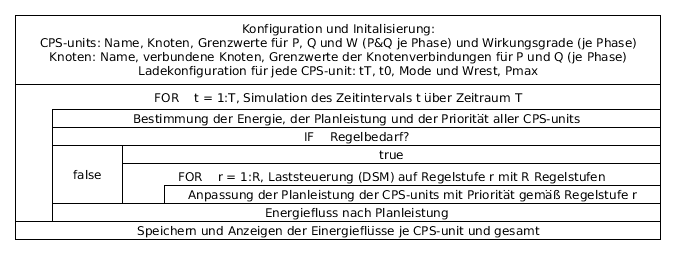
\includegraphics[width=14cm]{pap_dsm}
	\caption{Programmablaufplan zur Simulation der Energieflüsse einer teilautarken Ladeinfrastruktur}
	\label{Abb:Simulation_pap}
\end{figure} 	

%%%%%%%%%%%%%%%%%%%%%%%%%%%%%%%%%%%%%%%%%%%%%%%%%%%%%%%%%%%%%%%%%%%%%%%%%%%%%%%

\newpage
\section{Code Beispiele}
\label{Kap:Code}

  \subsection{weatheranalysis.m}
      \lstinputlisting[label=Code:weatheranalysis, caption=Programm $weatheranalysis$ zur Analyse von Globalstrahlungsdaten des DWD und Erstellung von Tagesertragsprofilen von PV-Anlagen]{./code/weatheranalysis.m}
  \subsection{energyflowsim.m}
      \lstinputlisting[label=Code:energyflowsim, caption=Programm $energyflowsim$ zur Simulation von Energieflüssen einer teilautarken Ladeinfrastruktur]{./code/energyflowsim.m}
  \subsection{dsmrel.m}
      \lstinputlisting[label=Code:DSM, caption=Beispiel Funktion für gleichmäßiges DSM]{./code/dsmrel.m}


\section{Konfigurationsdateien und PV-Ertragsdaten für energyflowsim.m}
\label{Kap:Konfiguration}

In diesem Kapitel sind die CSV-Konfigurationsdateien für den .m-Code gelistet. Tabelle \ref{Tab:cfg_cps} definiert die statischen Parameter für alle CPS-units und Tabelle \ref{Tab:cfg_node} für alle Knoten (nodes). Die mit $weatheranalysis.m$ unter den in Kapitel \ref{Kap4} definierten Randbedingungen generierten Ertragsdaten der PV-Module für die Szenarien Worst Case, Normal Case und Best Case sind in Tabelle \ref{Tab:cfg_pv_gen_all} aufgeführt. Die Usecases aller CPS-units für die drei genannten Szenarien sind in den Tabellen \ref{Tab:cfg_cpsuse_wc}, \ref{Tab:cfg_cpsuse_nc} und \ref{Tab:cfg_cpsuse_bc} parametrisiert.

		\begin{table}[h] 
			\centering
			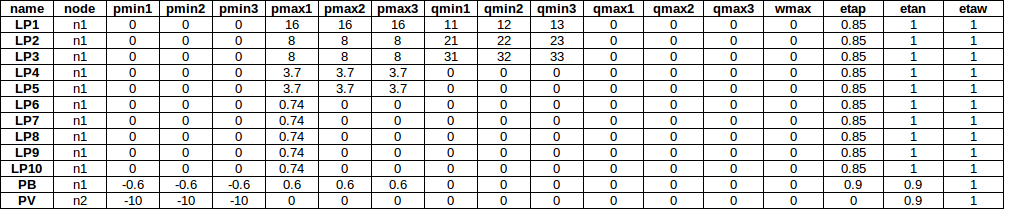
\includegraphics[width=14cm, height=5cm]{cfg_cps}
			\caption{Konfigurationsdatei für CPS-units: cfg\_cps.csv}
			\label{Tab:cfg_cps}
		\end{table} 
        
        \begin{table}[h] 
			\centering
			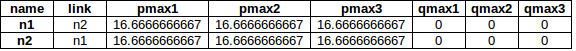
\includegraphics[width=14cm]{cfg_node}
			\caption{Konfigurationsdatei für Knoten: cfg\_node.csv}
			\label{Tab:cfg_node}
		\end{table} 

		\begin{wraptable}[h]{r}{7cm} 
			\centering
			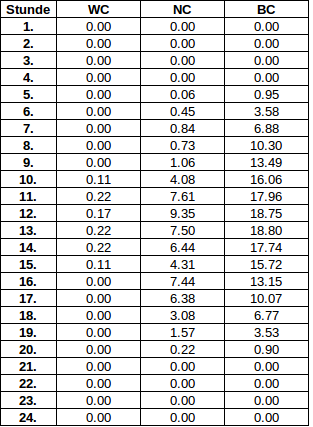
\includegraphics[width=7cm]{cfg_pv_gen_all}
			\caption{Stündliche Ertragsdaten der PV-Module in den Szenarien Worst, Normal und Bestcase in kWh}
			\label{Tab:cfg_pv_gen_all}
		\end{wraptable} 

        \begin{table}[h] 
			\centering
			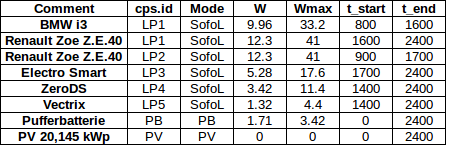
\includegraphics[width=14cm]{cfg_cpsuse_wc}
			\caption{Konfigurationsdatei für CPS Usecases im Worst Case: \\cfg\_cpsuse\_wc.csv}
			\label{Tab:cfg_cpsuse_wc}
		\end{table} 

        \begin{table}[h] 
			\centering
			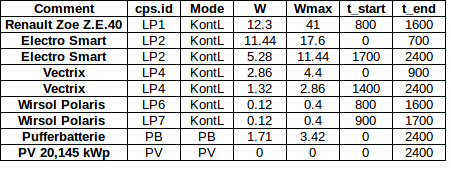
\includegraphics[width=14cm]{cfg_cpsuse_nc}
			\caption{Konfigurationsdatei für CPS Usecases im Normal Case: \\cfg\_cpsuse\_nc.csv}
			\label{Tab:cfg_cpsuse_nc}
		\end{table} 
        
        \begin{table}[h] 
			\centering
			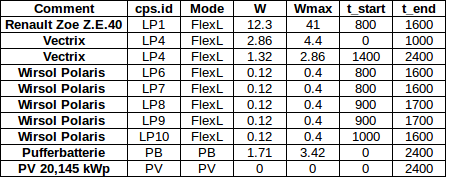
\includegraphics[width=14cm]{cfg_cpsuse_bc}
			\caption{Konfigurationsdatei für CPS Usecases im Best Case: \\cfg\_cpsuse\_bc.csv}
			\label{Tab:cfg_cpsuse_bc}
		\end{table} 

%------------------------------------------


        
        